\documentclass{standalone}
\usepackage{tikz}
\usepackage{amsmath}
\usetikzlibrary{automata,positioning,arrows,shapes.geometric, calc,patterns}

\begin{document}
	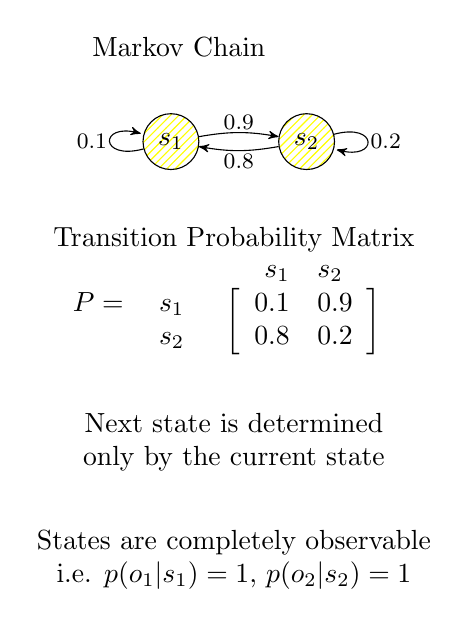
\begin{tikzpicture}[
		shaded/.style={draw,circle,pattern=north east lines, pattern color=yellow},
	    > = stealth',
		auto,
		prob/.style = {inner sep=1pt,font=\footnotesize}
		]
		% Markov Chain
		\node[shaded] at (0,0) (s1) {$s_1$};
		\node[shaded, right= of s1] (s2) {$s_2$};
		% Draw the causality arrows
		\path[->] 	(s1) edge [loop left] node[prob] {$0.1$}(s1)
					(s2) edge [loop right] node[prob] {$0.2$}(s2)
					(s1) edge [bend left=10] node[prob]{$0.9$} (s2)
					(s2) edge [bend left = 10] node[prob] {$0.8$}(s1);

		% denote
		\node[above = of s1,align=center,xshift= 1mm,yshift = -4mm]  {Markov Chain};
		\node[below = of s1,align=center,xshift= 8mm,yshift = 4mm] (TP)  { Transition Probability Matrix \\$
				P =
				\begin{array}{cc}
					& \begin{array}{cc} s_1 & s_2 \end{array} \\
					\begin{array}{c}
						s_1 \\
						s_2 \\
					\end{array}
					& \left[ \begin{array}{cc}
						0.1 & 0.9 \\
						0.8 & 0.2  \\
					\end{array} \right]
				\end{array}
				$};
		\node[below= of TP,align=center,xshift= 0mm,yshift = 5mm] (next) {Next state is determined \\ only by the current state};	
		\node[below= of next,align=center,xshift= 0mm,yshift = 5mm] (next) {States are completely observable\\i.e. $p(o_1|s_1) = 1$, $p(o_2|s_2) = 1$};	
	\end{tikzpicture}
	
	% Hidden Markov Model
	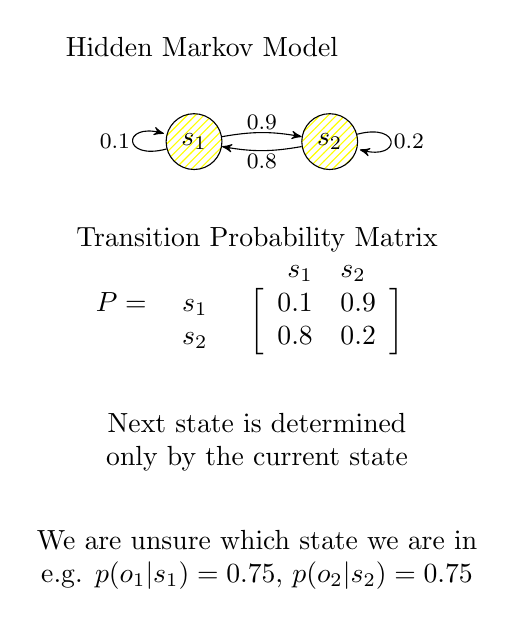
\begin{tikzpicture}[
		shaded/.style={draw,circle,pattern=north east lines, pattern color=yellow},
		> = stealth',
		auto,
		prob/.style = {inner sep=1pt,font=\footnotesize}
		]
		\node[shaded] at (0,0) (s1) {$s_1$};
		\node[shaded, right= of s1] (s2) {$s_2$};
		% Draw the causality arrows
		\path[->] 	(s1) edge [loop left] node[prob] {$0.1$}(s1)
		(s2) edge [loop right] node[prob] {$0.2$}(s2)
		(s1) edge [bend left=10] node[prob]{$0.9$} (s2)
		(s2) edge [bend left = 10] node[prob] {$0.8$}(s1);
		
		% denote
		\node[above = of s1,align=center,xshift= 1mm,yshift = -4mm]  {Hidden Markov Model};
		\node[below = of s1,align=center,xshift= 8mm,yshift = 4mm] (TP)  {Transition Probability Matrix \\$
			P =
			\begin{array}{cc}
				& \begin{array}{cc} s_1 & s_2 \end{array} \\
				\begin{array}{c}
					s_1 \\
					s_2 \\
				\end{array}
				& \left[ \begin{array}{cc}
					0.1 & 0.9 \\
					0.8 & 0.2  \\
				\end{array} \right]
			\end{array}
			$};
		\node[below= of TP,align=center,xshift= 0mm,yshift = 5mm] (next) {Next state is determined \\ only by the current state};
		\node[below= of next,align=center,xshift= 0mm,yshift = 5mm] (next) {We are unsure which state we are in \\e.g. $p(o_1|s_1) = 0.75$, $p(o_2|s_2) = 0.75$};	
	\end{tikzpicture}
	
	% Markov Decision Process
	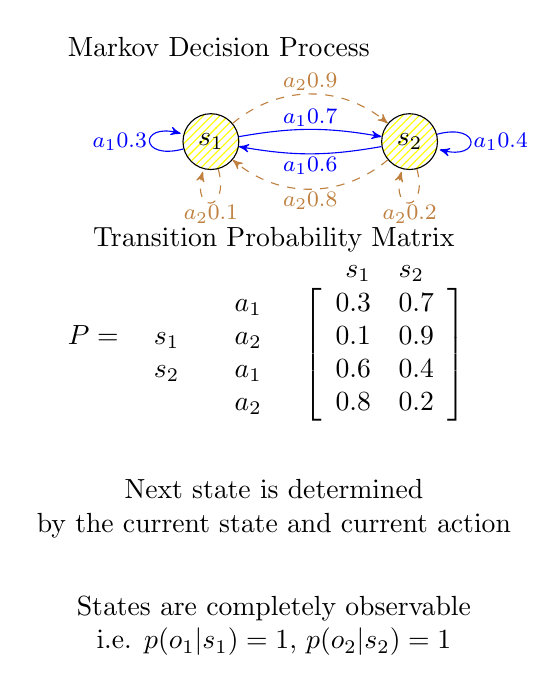
\begin{tikzpicture}[
		shaded/.style={draw,circle,pattern=north east lines, pattern color=yellow},
		> = stealth',
		auto,
		prob/.style = {inner sep=1pt,font=\footnotesize}
		]
		\node[shaded] at (0,0) (s1) {$s_1$};
		\node[shaded, right= of s1,xshift= 8mm] (s2) {$s_2$};
		% Draw the causality arrows
		\path[->] 	
		(s1) edge [loop left,blue] node[prob] {$a_1 0.3$}(s1)
		(s1) edge [loop below,brown,dashed] node[prob] {$a_2 0.1$}(s1)
		(s2) edge [loop right,blue] node[prob] {$a_1 0.4$}(s2)
		(s2) edge [loop below,brown,dashed] node[prob] {$a_2 0.2$}(s2)
		(s1) edge [bend left=10,blue] node[prob]{$a_1 0.7$} (s2)
		(s1) edge [bend left = 40,brown,dashed] node[prob]{$a_2 0.9$} (s2)
		(s2) edge [bend left = 10,blue] node[prob] {$a_1 0.6$}(s1)
		(s2) edge [bend left = 40,brown,dashed] node[prob] {$a_2 0.8$}(s1);
		
		% denote
		\node[above = of s1,align=center,xshift= 1mm,yshift = -4mm]  {Markov Decision Process};
		\node[below = of s1,align=center,xshift= 8mm,yshift = 4mm] (TP)  { Transition Probability Matrix \\$
			P =
			\begin{array}{ccc}
				&  &\begin{array}{cc} s_1 & s_2 \end{array} \\
				\begin{array}{c}
					s_1 \\
					s_2 
				\end{array} 
				&
				\begin{array}{c}
					a_1 \\
					a_2 \\
					a_1 \\
					a_2
				\end{array} 
				& \left[ \begin{array}{cc}
					0.3 & 0.7 \\
					0.1 & 0.9 \\
					0.6 & 0.4 \\
					0.8 & 0.2  
				\end{array} \right]
			\end{array}
			$};
		\node[below= of TP,align=center,xshift= 0mm,yshift = 5mm] (next) {Next state is determined \\ by the current state and current action};
		\node[below= of next,align=center,xshift= 0mm,yshift = 5mm] (next) {States are completely observable\\i.e. $p(o_1|s_1) = 1$, $p(o_2|s_2) = 1$};	
	\end{tikzpicture}
	
	% Partially Observable Markov Decision Process
	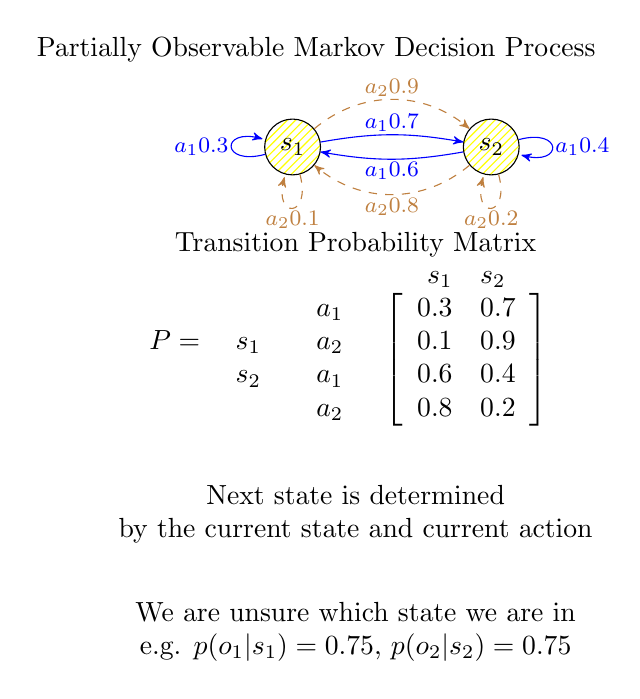
\begin{tikzpicture}[
		shaded/.style={draw,circle,pattern=north east lines, pattern color=yellow},
		> = stealth',
		auto,
		prob/.style = {inner sep=1pt,font=\footnotesize}
		]
		\node[shaded] at (0,0) (s1) {$s_1$};
		\node[shaded, right= of s1,xshift= 8mm] (s2) {$s_2$};
		% Draw the causality arrows
		\path[->] 	
		(s1) edge [loop left,blue] node[prob] {$a_1 0.3$}(s1)
		(s1) edge [loop below,brown,dashed] node[prob] {$a_2 0.1$}(s1)
		(s2) edge [loop right,blue] node[prob] {$a_1 0.4$}(s2)
		(s2) edge [loop below,brown,dashed] node[prob] {$a_2 0.2$}(s2)
		(s1) edge [bend left=10,blue] node[prob]{$a_1 0.7$} (s2)
		(s1) edge [bend left = 40,brown,dashed] node[prob]{$a_2 0.9$} (s2)
		(s2) edge [bend left = 10,blue] node[prob] {$a_1 0.6$}(s1)
		(s2) edge [bend left = 40,brown,dashed] node[prob] {$a_2 0.8$}(s1);
		
		% denote
		\node[above = of s1,align=center,xshift= 3mm,yshift = -4mm]  {Partially Observable Markov Decision Process};
		\node[below = of s1,align=center,xshift= 8mm,yshift = 4mm] (TP)  { Transition Probability Matrix \\$
			P =
			\begin{array}{ccc}
				&  &\begin{array}{cc} s_1 & s_2 \end{array} \\
				\begin{array}{c}
					s_1 \\
					s_2 
				\end{array} 
				&
				\begin{array}{c}
					a_1 \\
					a_2 \\
					a_1 \\
					a_2
				\end{array} 
				& \left[ \begin{array}{cc}
					0.3 & 0.7 \\
					0.1 & 0.9 \\
					0.6 & 0.4 \\
					0.8 & 0.2  
				\end{array} \right]
			\end{array}
			$};
		\node[below= of TP,align=center,xshift= 0mm,yshift = 5mm] (next) {Next state is determined \\ by the current state and current action};
		\node[below= of next,align=center,xshift= 0mm,yshift = 5mm] (next) {We are unsure which state we are in\\e.g. $p(o_1|s_1) = 0.75$, $p(o_2|s_2) = 0.75$};	
	\end{tikzpicture}
\end{document}
